\section{Kết quả và Phân tích}
\label{sec:ketqua}

Toàn bộ số liệu trong mục này trích xuất verbatim từ log thực thi tự động lưu tại \texttt{btl\_softsec/logs/} (sinh bởi \texttt{python run\_all.py}), không phải số liệu minh họa.

\subsection{Kết quả Chương 1 -- BMC}

\begin{table}[H]
  \centering
  \caption{Kết quả BMC $k=5$ trên 5 thuộc tính $P_1$--$P_5$}
  \label{tab:bmc}
  \small
  \begin{tabularx}{\linewidth}{@{}l X >{\centering\arraybackslash}p{2.6cm} >{\centering\arraybackslash}p{1.7cm}@{}}
    \toprule
    \textbf{Thuộc tính} & \textbf{Công thức} & \textbf{BUGGY} & \textbf{FIXED} \\
    \midrule
    $P_1$ Safety   & $G(\text{calculated}\to\text{assigned})$          & \textbf{SAT} -- counterexample qua $S_5$ (chi tiết dưới bảng) & \textbf{UNSAT} \checkmark \\
    $P_2$ Safety   & $G(\text{exported}\to\text{calculated})$          & \textbf{UNSAT} \checkmark & \textbf{UNSAT} \checkmark \\
    $P_3$ Liveness & $G(\text{assigned}\to F\,\text{calculated})$      & \textbf{SAT} ($k{=}5$ limit) & \textbf{SAT} ($k{=}5$ limit) \\
    $P_4$ Safety   & $G(\text{error}\to\lnot\,\text{exported})$        & \textbf{UNSAT} \checkmark & \textbf{UNSAT} \checkmark \\
    $P_5$ Safety   & $G(\text{exported}\to\lnot\,\text{byte\_truncated})$ & \textbf{SAT} -- qua $S_{2B}$ (chi tiết dưới bảng) & \textbf{UNSAT} \checkmark \\
    \bottomrule
  \end{tabularx}
\end{table}

Mô hình FIXED hiện có \textbf{6 trạng thái} ($S_0,S_1,S_{2A},S_{2B},S_3,S_4$) và bản BUGGY có \textbf{7 trạng thái} (thêm $S_5$) -- xem \Cref{sec:ch1} để biết vì sao $S_2$ SALARY\_CALC gốc được tách thành $S_{2A}$/$S_{2B}$. Việc tách này không làm đổi bất kỳ kết quả SAT/UNSAT nào ở trên so với mô hình gốc (đã xác nhận bằng cách chạy lại BMC sau khi sửa).

\textbf{Counterexample trace thật} cho $P_1$ trên bản BUGGY (\texttt{logs/kripke\_bmc.log}):
\begin{quote}\ttfamily\footnotesize
Step 0: S0\_INIT [init] $\to$ Step 1: S5\_INVALID\_CALC [calculated,error] $\to$ Step 2: S4\_ERROR [error] \\
$\to$ Step 3: S0\_INIT [init] $\to$ Step 4: S1\_GV\_ASSIGNED [assigned] \\
$\to$ Step 5: S2A\_CALC\_THUONG [assigned,calculated,lop\_thuong]
\end{quote}

\textbf{Counterexample trace thật} cho $P_5$ trên bản BUGGY (\texttt{logs/kripke\_bmc.log}) -- nay đi qua đúng nhánh $S_{2B}$ CALC\_DONG (lớp đông, statement \Cref{sec:params}):
\begin{quote}\ttfamily\footnotesize
Step 0: S0\_INIT [init] $\to$ Step 1: S1\_GV\_ASSIGNED [assigned] $\to$ Step 2: S2B\_CALC\_DONG [assigned,calculated,lop\_dong] \\
$\to$ Step 3: S3\_EXPORTED [assigned,byte\_truncated,calculated,exported] \\
$\to$ Step 4: S0\_INIT [init] $\to$ Step 5: S1\_GV\_ASSIGNED [assigned]
\end{quote}

$P_3$ ra \textbf{SAT} ở cả 2 bản -- đây \emph{không phải lỗi mã nguồn}, mà là giới hạn kỹ thuật tự nhiên của BMC hữu hạn $k=5$ đối với thuộc tính Liveness (cần $k$-induction hoặc Büchi automata để chứng minh liveness vô hạn triệt để).

\subsection{Kết quả Chương 2 -- 9 findings}

\begin{table}[H]
  \centering
  \caption{Toàn bộ 9 cảnh báo phát hiện bởi \texttt{pattern\_scanner.py} trên code VULN; \texttt{main\_fixed.c} sạch tuyệt đối (0 finding)}
  \label{tab:findings}
  \small
  \begin{tabularx}{\linewidth}{@{}l l l X@{}}
    \toprule
    \textbf{Vị trí} & \textbf{CWE} & \textbf{Rule} & \textbf{Mức độ} \\
    \midrule
    \texttt{giang\_vien.c:12}     & CWE-120 & \texttt{strcpy}                    & HIGH \\
    \texttt{giang\_vien.c:15}     & CWE-120 & \texttt{strcpy} (\texttt{hoTen})    & HIGH \\
    \texttt{giang\_vien.c:18}     & CWE-120 & \texttt{strcpy} (\texttt{bangCap})  & HIGH \\
    \texttt{giang\_vien.c:35}     & CWE-416 & \texttt{dangling\_free}             & HIGH \\
    \texttt{lop\_hoc\_phan.c:13}  & CWE-120 & \texttt{strcpy} (\texttt{maLop})    & HIGH \\
    \texttt{tinh\_tien\_day.c:12} & CWE-190 & \texttt{int\_overflow\_cast}        & HIGH \\
    \texttt{tinh\_tien\_day.c:13} & CWE-190 & \texttt{int\_overflow\_cast}        & HIGH \\
    \texttt{tinh\_tien\_day.c:13} & CWE-476 & \texttt{unchecked\_nested\_deref}   & HIGH \\
    \texttt{tinh\_tien\_day.c:68} & CWE-197 & \texttt{unchecked\_numeric\_truncation} & HIGH \\
    \bottomrule
  \end{tabularx}
\end{table}

Điểm đáng chú ý: \texttt{pack\_class\_size\_byte\_SAFE()} nằm \emph{trong cùng file} \texttt{tinh\_tien\_day.c} với hàm VULN nhưng \textbf{không} bị báo động giả, vì scanner tìm thấy đúng guard \texttt{if (soLuongSinhVien < 0 || > 127)} trong phạm vi hàm bao quanh -- xác nhận cơ chế xét theo hàm (không phải theo tên file) hoạt động đúng.

\Cref{lst:delvuln,lst:delsafe} trích nguyên văn cặp hàm gây ra và khắc phục CWE-416 (dòng \texttt{giang\_vien.c:35} trong \Cref{tab:findings}): bản VULN \texttt{free(gv)} mà không huỷ liên kết \texttt{gv\_ptr} ở Module 2; bản SAFE nhận tham số \texttt{GiangVien **} để có thể tự đặt con trỏ gốc về \texttt{NULL} ngay sau khi giải phóng.

\lstinputlisting[language=C,firstline=32,lastline=37,caption={\texttt{delete\_lecturer\_VULN()} -- CWE-416: \texttt{free()} không huỷ liên kết},label={lst:delvuln}]{code/giang_vien.c}

\lstinputlisting[language=C,firstline=71,lastline=77,caption={\texttt{delete\_lecturer\_SAFE()} -- khắc phục: nhận \texttt{GiangVien **} để nullify con trỏ gốc},label={lst:delsafe}]{code/giang_vien.c}

\Cref{lst:packvuln,lst:packsafe} trích nguyên văn cặp hàm CWE-197 (dòng \texttt{tinh\_tien\_day.c:68} trong \Cref{tab:findings}), đúng cặp hàm được chứng minh hình thức ở Check 4/5 (\Cref{sec:ch3}).

\lstinputlisting[language=C,firstline=67,lastline=69,caption={\texttt{pack\_class\_size\_byte\_VULN()} -- CWE-197: ép kiểu không kiểm tra phạm vi},label={lst:packvuln}]{code/tinh_tien_day.c}

\lstinputlisting[language=C,firstline=75,lastline=82,caption={\texttt{pack\_class\_size\_byte\_SAFE()} -- khắc phục: guard \texttt{[0,127]} trước khi ép kiểu},label={lst:packsafe}]{code/tinh_tien_day.c}

\subsection{Kết quả kiểm chứng NFR-1/NFR-2 (\texttt{nfr\_check.py})}

Bổ sung cho \Cref{tab:nfr}: subcommand \texttt{e2e\_nfr\_bench} (mới thêm vào \texttt{main.c}/\texttt{main\_fixed.c}) đo \emph{thực nghiệm} 2 yêu cầu phi chức năng quan trọng nhất, chạy $N=10\,000$ lần trên chính 2 binary đã biên dịch của Chương 2 (không phải microbenchmark tách biệt):

\begin{itemize}
  \item \textbf{NFR-1 (Hiệu năng)}: trung bình $0{,}000014\,$ms/lần gọi \texttt{calculate\_\allowbreak e2e\_\allowbreak salary\_\allowbreak SAFE()} ($0{,}000011\,$ms/lần trên bản VULN) -- thấp hơn ngưỡng $10\,$ms gần $6$ bậc độ lớn -- \textbf{PASS}.
  \item \textbf{NFR-2 (Ổn định bộ nhớ)}: sau $10\,000$ lần tạo/xoá \texttt{GiangVien}+\texttt{LopHocPhan} liên tục, \texttt{WorkingSetSize} (đo qua \texttt{GetProcessMemoryInfo}) chỉ trôi $4$\,KB trên cả bản SAFE và bản VULN (ngưỡng $1024$\,KB) -- \textbf{PASS cả 2 bản}. Kết quả này \emph{nhất quán với lý thuyết} nêu ở \Cref{sec:thaoluan}: CWE-416 trong đề tài là lỗi con trỏ treo (dangling pointer, \texttt{gv\_ptr} vẫn trỏ tới vùng nhớ đã \texttt{free()}), không phải rò rỉ bộ nhớ (memory leak) -- cả \texttt{delete\_lecturer\_VULN()} lẫn \texttt{delete\_lecturer\_SAFE()} đều gọi \texttt{free()} đầy đủ, nên không có gì để rò rỉ; hai lớp lỗi bộ nhớ này độc lập với nhau.
\end{itemize}

Toàn bộ số liệu trích \emph{verbatim} từ \texttt{logs/nfr\_check.log} -- trước khi có subcommand này, NFR-1/NFR-2 chỉ được biện luận gián tiếp (công thức $O(1)$, 0/200 crash), chưa có phép đo trực tiếp ở đúng quy mô $10^4$ đã đặc tả.

\subsection{Kết quả Chương 3 -- SMT}

\begin{itemize}
  \item \textbf{Check 1 SAT}: counterexample $\text{numClasses}=20$, $\text{soTiet}=120$, $\text{soLuongSinhVien}=0$ (nên $\text{heSoQuyMo}=0.0$, đúng statement \Cref{sec:params}), $\text{heSoHocPhan}\approx 3.0$, $\text{heSoBangCap}\approx 2.0$, $\text{dinhMucTienChuan}=149\,131$ VNĐ $\Rightarrow$ tổng thù lao vượt \texttt{INT32\_MAX}. (Đã sửa mô hình để dùng đúng \texttt{soLuongSinhVien} thật thay cho biến tự do \texttt{heSoQuyMoLop} không tồn tại trong code -- xem \Cref{sec:params}; kết luận SAT không đổi.)
  \item \textbf{Check 2 UNSAT}: chứng minh \texttt{long long} an toàn tuyệt đối trong toàn bộ ràng buộc doanh nghiệp ($\text{numClasses}\in[1,100]$, $\text{dinhMucTienChuan}$ tới 2 triệu VNĐ).
  \item \textbf{Check 3 UNSAT}: guard-check (\texttt{gv\_ptr} NULL/đã xóa $\to$ lương $=0$) hoạt động đúng trên chính công thức thật.
  \item \textbf{Check 4 SAT}: phản ví dụ $\text{soLuongSinhVien}=128 \to \text{byte}=-128$.
  \item \textbf{Check 5 UNSAT}: với guard $[0,127]$ đúng trước, ép kiểu không bao giờ sai lệch.
  \item \textbf{Check 6 SAT}: $a=0$ (lớp rỗng thật) và $b=256$ (lớp có thật 256 sinh viên) đều cho byte $=0$ -- 2 tình huống nghiệp vụ hoàn toàn khác nhau không thể phân biệt sau khi xuất báo cáo.
  \item \textbf{Check 7 SAT} (mới, CWE-1288): giảng viên \texttt{CU\_NHAN} thật và 1 chuỗi \texttt{bangCap} không hợp lệ đều cho $\text{heSoBangCap}=1.0$ -- cùng lớp lỗi ``va chạm trạng thái'' như Check 6, nhưng ở Module 1 (xem \Cref{sec:quytrinh}); khác CWE-197, lỗi này không thể loại trừ hoàn toàn bằng cách từ chối (nghiệp vụ cần 1 giá trị fallback thật), bản SAFE chỉ thêm được cảnh báo phát hiện.
\end{itemize}

\subsection{Kết quả Chương 4 -- Fuzzing}

\begin{table}[H]
  \centering
  \caption{So sánh Black-box vs. White-box (lần chạy đại diện, \texttt{logs/fuzzer\_black/whitebox.log})}
  \label{tab:fuzz}
  \small
  \begin{tabular}{@{}l c c@{}}
    \toprule
    \textbf{Tiêu chí} & \textbf{Black-box} & \textbf{White-box (Z3)} \\
    \midrule
    Số lần thử                & 200 (ngẫu nhiên)      & 7 (giải trực tiếp) \\
    Số crash phát hiện (VULN) & 72/200 (36.0\%)       & 7/7 target (100\%) \\
    Số crash (SAFE)           & 0/200                 & -- \\
    Thời gian thực thi        & 9.86 s                & 0.3412 s \\
    Tốc độ tăng tốc           & mức cơ sở             & $\approx 28.9\times$ nhanh hơn \\
    \bottomrule
  \end{tabular}
\end{table}

\begin{figure}[H]
  \centering
  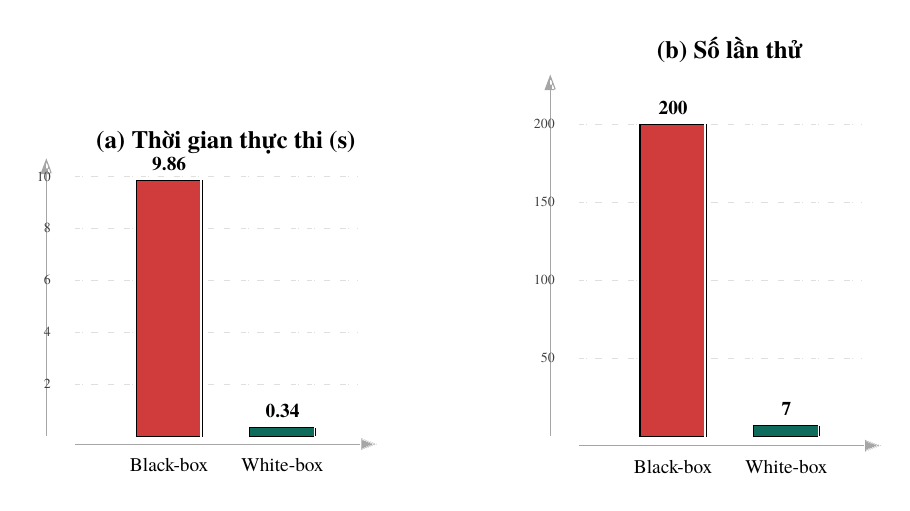
\includegraphics[width=\linewidth]{diagram5_fuzz_compare.png}
  \caption{Black-box vs. White-box: (a) thời gian thực thi và (b) số lần thử cần để phát hiện đủ lỗ hổng đã biết (số liệu khớp \protect\Cref{tab:fuzz})}
  \label{fig:fuzz-bar}
\end{figure}

Hai biểu đồ trên cùng minh họa một kết luận: White-box (thanh xanh, giải trực tiếp ràng buộc Z3) đạt \textbf{cùng độ chính xác 100\% trên 7 mục tiêu} chỉ với 7 lần thử và 0.34s, trong khi Black-box (thanh đỏ, sinh input ngẫu nhiên) cần 200 lần thử và 9.86s -- chênh lệch trực quan $\approx 28.9\times$ về thời gian mà không cần đọc số trong \Cref{tab:fuzz}. (Thời gian đo bằng wall-clock thật nên dao động nhẹ giữa các lần chạy tuỳ tải máy -- số crash/SAT ở trên mới là bằng chứng chính, không phải số giây tuyệt đối.)

Riêng CWE-197 (không biểu hiện bằng crash mà bằng sai lệch dữ liệu âm thầm): black-box ngẫu nhiên cho \textbf{120/200 (60\%)} sai lệch trên bản VULN, \textbf{0/200} trên bản SAFE (146/200 bị chặn an toàn). Bộ 17 giá trị biên (BVA) tất định khớp \textbf{17/17 (100\%)} giữa byte thật và byte tính tay trên cả 2 bản, và tự động lộ ra \textbf{6 nhóm trùng lặp byte} trên bản VULN (ví dụ byte $=0$ được tạo bởi cả 3 giá trị $-256, 0, 256$), \textbf{0 nhóm} trên bản SAFE.

\subsection{Bảng tổng hợp CWE và mức độ rủi ro (CVSS-lite)}

Điểm CVSS-lite~\cite{cvss31} dưới đây được tính theo công thức $\text{Score} = \min(\text{Exploitability} + \text{Impact}, 10)$ với $\text{Exploitability} = 8.22 \times AV \times AC \times PR \times UI$ và $\text{Impact} = 6.42\times(1-(1-C)(1-I)(1-A))$ (cùng mô hình CVSS-lite đã dùng ở \texttt{lab3\_secure\_memory}), áp dụng $AV{=}$Local (chương trình CLI cục bộ, không phải dịch vụ mạng), $AC{=}$Low, $PR{=}$None, $UI{=}$None cho toàn bộ 6 CWE, và mức Impact (C/I/A) lấy theo đúng hậu quả \emph{đã chứng minh được bằng thực nghiệm} ở các mục trên (không giả định RCE chưa kiểm chứng).

\begin{table}[H]
  \centering
  \caption{Tổng hợp CWE, vị trí trong đề tài và điểm CVSS-lite tự tính}
  \label{tab:cwe-cvss}
  \small
  \begin{tabularx}{\linewidth}{@{}l X c l@{}}
    \toprule
    \textbf{CWE} & \textbf{Vị trí trong đề tài} & \textbf{CVSS-lite} & \textbf{Mức} \\
    \midrule
    CWE-120~\cite{cwe120}   & Ch2 \texttt{strcpy}; Ch4 crash 72/200            & 7.2 & HIGH \\
    CWE-416~\cite{cwe416}   & Ch2 \texttt{dangling\_free}; Ch2.1 ASan \texttt{heap-use-after-free} thật & 8.0 & HIGH \\
    CWE-476~\cite{cwe476}   & Ch2 \texttt{unchecked\_nested\_deref}; Ch4 Target 4 & 6.7 & MEDIUM \\
    CWE-190~\cite{cwe190}   & Ch1 $S_5$; Ch3 Check 1 SAT / Check 2 UNSAT       & 6.1 & MEDIUM \\
    CWE-197~\cite{cwe197}   & Ch1 $P_5$; Ch3 Check 4/6; Ch4 BVA 17/17          & 6.1 & MEDIUM \\
    CWE-1288~\cite{cwe1288} & Ch2 fallback \texttt{heSoBangCap=1.0f}; Ch3 Check 7 SAT & 3.9 & LOW \\
    \bottomrule
  \end{tabularx}
\end{table}

\begin{figure}[H]
  \centering
  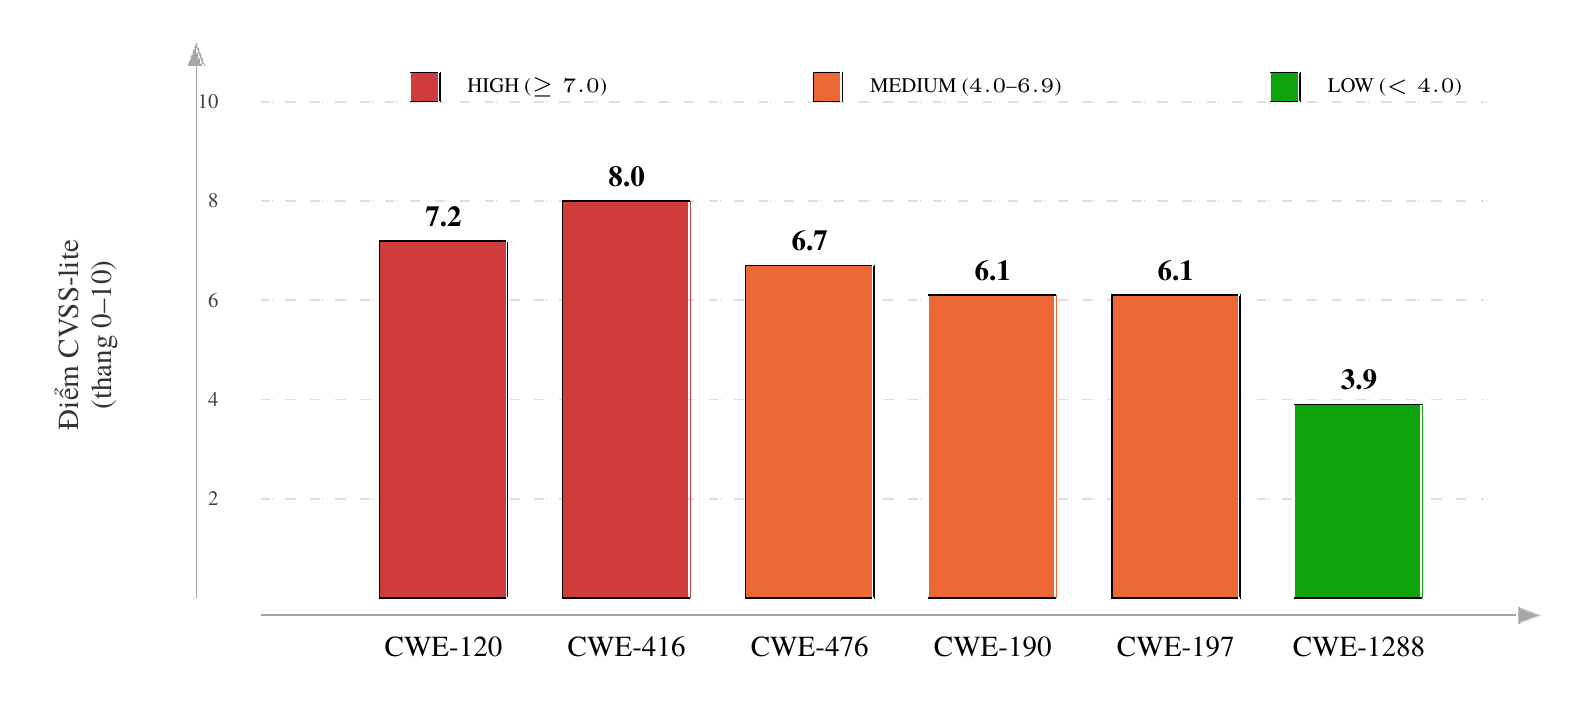
\includegraphics[width=0.85\linewidth]{diagram4_cvss_bar.png}
  \caption{So sánh điểm CVSS-lite giữa 6 CWE của đề tài (số liệu khớp \protect\Cref{tab:cwe-cvss})}
  \label{fig:cvss-bar}
\end{figure}

Nhìn theo biểu đồ: CWE-416 (UAF) và CWE-120 (buffer overflow) là 2 lớp lỗi nghiêm trọng nhất (HIGH, $\geq 7.0$) -- đúng với trực giác vì cả 2 đều có thể dẫn tới hỏng bộ nhớ ngay lập tức; CWE-197 và CWE-190 tuy nguy hiểm nhưng ở mức MEDIUM vì hậu quả quan sát được (sai lệch dữ liệu/DoS) chưa được chứng minh leo thang tới RCE trong phạm vi đề tài (xem hướng mở rộng ở \Cref{sec:thaoluan}).

\begin{table}[H]
  \centering
  \caption{Ví dụ thực tế minh họa cho mỗi lớp CWE}
  \label{tab:cwe-examples}
  \small
  \begin{tabularx}{\linewidth}{@{}l X@{}}
    \toprule
    \textbf{CWE} & \textbf{Ví dụ thực tế minh họa} \\
    \midrule
    CWE-120  & CVE-2003-0352~\cite{cve2003-0352} -- lỗi tràn bộ đệm trong Windows RPC DCOM, bị khai thác bởi worm Blaster \\
    CWE-416  & CVE-2019-0708~\cite{cve2019-0708} (``BlueKeep'') -- use-after-free trong Windows Remote Desktop Services \\
    CWE-476  & Điển hình lớp lỗi DoS phổ biến; xem thêm các ví dụ tại trang CWE-476 của MITRE~\cite{cwe476} \\
    CWE-190  & Ariane 5 Flight 501 (1996)~\cite{ariane5report} -- không phải mã CVE (xảy ra trước khi hệ thống CVE ra đời năm 1999) nhưng là sự cố tràn số nguyên kinh điển nhất từng được ghi nhận \\
    CWE-197  & Chưa xác minh được một CVE công khai khớp chính xác; xem trang CWE-197 của MITRE~\cite{cwe197} \\
    CWE-1288 & Chưa xác minh được một CVE công khai khớp chính xác; xem trang CWE-1288 của MITRE~\cite{cwe1288} \\
    \bottomrule
  \end{tabularx}
\end{table}

\noindent\textit{Lưu ý phương pháp luận:} bảng trên cố ý \textbf{không} gán một mã CVE cụ thể cho CWE-476/197/1288 vì không xác minh được một CVE thực sự khớp chính xác với bối cảnh đề tài trong phạm vi kiểm chứng cho phép -- thà để trống còn hơn trích dẫn một mã CVE không chắc chắn đúng.

\subsection{Ma trận truy vết Test Case $\to$ Yêu cầu (IEEE 829)}
\label{sec:traceability}

Các mục 5.1--5.4 trên trình bày kết quả \emph{theo từng chương/kỹ thuật}. Bảng dưới đây tổ chức lại đúng cùng số liệu đó theo hướng ngược lại -- \emph{theo từng yêu cầu (REQ/NFR)} -- theo tinh thần đặc tả \emph{Test Case Specification} của chuẩn IEEE~829-2008~\cite{ieee829} (mã test case, điều kiện đầu vào, kết quả mong đợi, kết quả thực tế đối chiếu ngược lại nguồn log thật). Đây là góc nhìn truy vết hai chiều REQ $\leftrightarrow$ Test Case còn thiếu ở \Cref{sec:dacta}, nơi mới chỉ đặc tả yêu cầu mà chưa chỉ rõ từng yêu cầu được kiểm chứng bởi test case cụ thể nào.

{\scriptsize
\setlength{\tabcolsep}{3.5pt}
\renewcommand{\arraystretch}{1.35}
\begin{longtable}{@{}
  >{\raggedright\arraybackslash}p{1.3cm}
  >{\raggedright\arraybackslash}p{1.2cm}
  >{\raggedright\arraybackslash}p{3.8cm}
  >{\raggedright\arraybackslash}p{2.3cm}
  >{\raggedright\arraybackslash}p{4.6cm}
  >{\centering\arraybackslash}p{1.1cm}@{}}
  \caption{Ma trận truy vết Test Case $\to$ Yêu cầu (mọi kết quả thực tế trích từ \texttt{logs/*.log} thật)}
  \label{tab:trace} \\
  \toprule
  \textbf{Mã TC} & \textbf{REQ} & \textbf{Input / Điều kiện} & \textbf{Kỳ vọng} & \textbf{Thực tế (nguồn log)} & \textbf{KL} \\
  \midrule
  \endfirsthead
  \multicolumn{6}{l}{\textit{(tiếp theo Bảng~\ref{tab:trace})}} \\
  \toprule
  \textbf{Mã TC} & \textbf{REQ} & \textbf{Input / Điều kiện} & \textbf{Kỳ vọng} & \textbf{Thực tế (nguồn log)} & \textbf{KL} \\
  \midrule
  \endhead
  \midrule
  \multicolumn{6}{r}{\textit{xem tiếp trang sau}} \\
  \endfoot
  \bottomrule
  \endlastfoot
  TC-K1-01 & REQ-1 & BMC $P_1$, bản BUGGY (bước nhảy thẳng sang tính tiền, bỏ qua phân công) & UNSAT (không vi phạm) & \textbf{SAT} -- phản ví dụ $S_0{\to}S_5{\to}S_4$ (\texttt{kripke\_bmc.log}) & FAIL$^*$ \\
  \addlinespace[3pt]
  TC-K1-02 & REQ-1 & BMC $P_1$, bản FIXED & UNSAT & UNSAT (\texttt{kripke\_bmc.log}) & PASS \\
  \addlinespace[3pt]
  TC-K1-03 & REQ-2 & BMC $P_2$, cả 2 bản & UNSAT & UNSAT cả 2 bản (\texttt{kripke\_bmc.log}) & PASS \\
  \addlinespace[3pt]
  TC-K2-01 & REQ-3 & Scanner quét \texttt{strcpy} (\texttt{hoTen}\slash\texttt{maLop}\slash\texttt{bangCap}\slash\texttt{maGiangVien}) trên 3 file VULN & Phát hiện đủ cảnh báo CWE-120 & 5 cảnh báo CWE-120 đúng vị trí (\texttt{pattern\_scanner.log}) & PASS \\
  \addlinespace[3pt]
  TC-K2-02 & REQ-3 & Scanner quét \texttt{main\_fixed.c} & 0 cảnh báo & 0 cảnh báo -- \texttt{[CLEAN]} (\texttt{pattern\_scanner.log}) & PASS \\
  \addlinespace[3pt]
  TC-K4-01 & REQ-3 & White-box Target 1: \texttt{hoTen} dài 81 ký tự $>$ CON-1 (80) & Tìm điều kiện gây tràn & SAT ở lần thử 1 (\texttt{fuzzer\_whitebox.log}) & FAIL$^*$ \\
  \addlinespace[3pt]
  TC-K4-02 & REQ-3 & White-box Target 2: \texttt{maLop} dài 21 ký tự $>$ CON-4 (20) & Tìm điều kiện gây tràn & SAT ở lần thử 2 (\texttt{fuzzer\_whitebox.log}) & FAIL$^*$ \\
  \addlinespace[3pt]
  TC-K4-03 & REQ-3 & Black-box 200 lần ngẫu nhiên trên VULN & 0/200 crash & 72/200 crash, exit \texttt{0xC0000374} (\texttt{fuzzer\_blackbox.log}) & FAIL$^*$ \\
  \addlinespace[3pt]
  TC-K4-04 & REQ-3 & Black-box 200 lần trên FIXED & 0/200 crash & 0/200 crash (\texttt{fuzzer\_blackbox.log}) & PASS \\
  \addlinespace[3pt]
  TC-K2-03 & REQ-4 & Scanner quét \texttt{dangling\_free} trên VULN & Phát hiện CWE-416 tại \texttt{giang\_vien.c:35} & Phát hiện đúng vị trí (\texttt{pattern\_scanner.log}) & PASS \\
  \addlinespace[3pt]
  TC-K4-05 & REQ-4 & White-box Target 3: \texttt{free(gv)} rồi vẫn đọc qua \texttt{gv\_ptr} & Tìm điều kiện UAF & SAT ở lần thử 3 (\texttt{fuzzer\_whitebox.log}) & FAIL$^*$ \\
  \addlinespace[3pt]
  TC-K2-04 & REQ-4 & \texttt{memory\_trace\_demo.py}: đọc \texttt{gv->hoTen} sau \texttt{free()}, bản ASan-VULN & ASan phải bắt lỗi & \texttt{heap-use-after-free}, ABORTING, offset $+24$ byte $=$ \texttt{hoTen} (\texttt{memory\_trace.log}) & FAIL$^*$ \\
  \addlinespace[3pt]
  TC-K2-05 & REQ-4 & \texttt{memory\_trace\_demo.py}, bản ASan-FIXED (\texttt{gv\_ptr=NULL} trước free) & 0 vi phạm & 0 vi phạm (\texttt{memory\_trace.log}) & PASS \\
  \addlinespace[3pt]
  TC-K2-06 & REQ-5 & Scanner quét \texttt{unchecked\_\allowbreak nested\_\allowbreak deref} trên VULN & Phát hiện CWE-476 tại \texttt{tinh\_tien\_day.c:13} & Phát hiện đúng vị trí (\texttt{pattern\_scanner.log}) & PASS \\
  \addlinespace[3pt]
  TC-K4-06 & REQ-5 & White-box Target 4: \texttt{gv\_ptr=NULL} rồi gọi \texttt{calculate\_e2e\_salary} & Tìm điều kiện NULL deref & SAT ở lần thử 4 (\texttt{fuzzer\_whitebox.log}) & FAIL$^*$ \\
  \addlinespace[3pt]
  TC-K3-01 & REQ-6 & Check 1 (Z3): $\exists$ input hợp lệ làm tràn \texttt{int32} & SAT dự kiến (đang kiểm định code VULN) & SAT -- numClasses=20, soTiet=120 (\texttt{smt\_verify.log}) & FAIL$^*$ \\
  \addlinespace[3pt]
  TC-K3-02 & REQ-6 & Check 2 (Z3): cùng câu hỏi trên \texttt{long long} (bản vá) & UNSAT & UNSAT (\texttt{smt\_verify.log}) & PASS \\
  \addlinespace[3pt]
  TC-K4-07 & REQ-6 & White-box Target 5: soTiet=16694179, dmt=2147583020 & SAT dự kiến & SAT ở lần thử 5 (\texttt{fuzzer\_whitebox.log}) & FAIL$^*$ \\
  \addlinespace[3pt]
  TC-K1-04 & REQ-8 & BMC $P_5$, bản VULN & UNSAT & SAT -- $S_3$ mang nhãn \texttt{byte\_truncated} (\texttt{kripke\_bmc.log}) & FAIL$^*$ \\
  \addlinespace[3pt]
  TC-K1-05 & REQ-8 & BMC $P_5$, bản FIXED & UNSAT & UNSAT (\texttt{kripke\_bmc.log}) & PASS \\
  \addlinespace[3pt]
  TC-K3-03 & REQ-8 & Check 4 (Z3): $\exists\, n\in[0,300]$ ép kiểu \texttt{char} sai giá trị & SAT dự kiến & SAT -- $n=128 \to$ byte $=-128$ (\texttt{smt\_verify.log}) & FAIL$^*$ \\
  \addlinespace[3pt]
  TC-K3-04 & REQ-8 & Check 5 (Z3): cùng câu hỏi với guard $[0,127]$ & UNSAT & UNSAT (\texttt{smt\_verify.log}) & PASS \\
  \addlinespace[3pt]
  TC-K3-05 & REQ-8, NFR-5 & Check 6 (Z3): $\exists\, a\ne b \in [0,300]$ cùng cho 1 byte & UNSAT mong muốn (an toàn truy vết) & SAT -- $a=0, b=256$ cùng byte $=0$ (\texttt{smt\_verify.log}) & FAIL$^{**}$ \\
  \addlinespace[3pt]
  TC-K4-08 & REQ-8 & Black-box CWE-197, 200 lần trên VULN & 0/200 sai lệch & 120/200 sai lệch, 60\% (\texttt{fuzzer\_blackbox.log}) & FAIL$^*$ \\
  \addlinespace[3pt]
  TC-K4-09 & REQ-8 & Black-box CWE-197, 200 lần trên FIXED & 0/200 sai lệch & 0/200 sai lệch, 146/200 chặn an toàn (\texttt{fuzzer\_blackbox.log}) & PASS \\
  \addlinespace[3pt]
  TC-K4-10 & REQ-8, NFR-5 & BVA 17 giá trị biên cố định trên VULN & Byte thật khớp byte tính tay 17/17; không nên trùng lặp & 17/17 khớp lý thuyết, nhưng lộ 6 nhóm trùng lặp byte thật (\texttt{fuzzer\_blackbox.log}) & PASS\slash FAIL$^{**}$ \\
  \addlinespace[3pt]
  TC-K4-11 & REQ-8, NFR-5 & BVA 17 giá trị biên trên FIXED & 0 nhóm trùng lặp & 0 nhóm trùng lặp (\texttt{fuzzer\_blackbox.log}) & PASS \\
  \addlinespace[3pt]
  TC-K3-06 & REQ-9 & Check 7 (Z3): $\exists$ 2 danh mục \texttt{bangCap} khác nhau (\texttt{CU\_NHAN} thật, chuỗi không hợp lệ) cùng cho 1 \texttt{heSoBangCap} & UNSAT mong muốn (phân biệt được) & SAT -- cả 2 cùng rơi vào fallback $1.0$ (\texttt{smt\_verify.log}) & FAIL$^{**}$ \\
  \addlinespace[3pt]
  TC-K4-12 & REQ-9 & Black-box: \texttt{bangCap} ngẫu nhiên gồm giá trị không hợp lệ, trên VULN & Cần oracle xác nhận hệ thống xử lý đúng & Script chỉ đếm 74/200 lần input không hợp lệ được sinh ra (không crash), KHÔNG assert hành vi đúng/sai (\texttt{fuzzer\_blackbox.log}) & QS$^\dagger$ \\
  \addlinespace[3pt]
  TC-K2-07 & REQ-7 & (chưa có test case riêng) & Công thức tính lương đúng với mọi input hợp lệ & Check 1/2 chỉ chứng minh KHÔNG TRÀN SỐ, không chứng minh giá trị tính ra khớp công thức nghiệp vụ mong đợi & QS$^\dagger$ \\
  \addlinespace[3pt]
  TC-N01 & NFR-1 & \texttt{e2e\_nfr\_bench 10000} trên \texttt{salary\_calc\_fixed.exe} (\texttt{QueryPerformanceCounter}) & Trung bình $<10\,$ms/lần & $0{,}000014\,$ms/lần (\texttt{nfr\_check.log}) & PASS \\
  \addlinespace[3pt]
  TC-N02 & NFR-1 & \texttt{e2e\_nfr\_bench 10000} trên \texttt{salary\_calc.exe} (VULN, đối chứng) & Trung bình $<10\,$ms/lần & $0{,}000011\,$ms/lần (\texttt{nfr\_check.log}) & PASS \\
  \addlinespace[3pt]
  TC-N03 & NFR-2 & $10\,000$ lần tạo/xoá \texttt{GiangVien}+\texttt{LopHocPhan} trên bản FIXED, đo \texttt{GetProcessMemoryInfo} & Drift $<1024$\,KB & Drift $=4$\,KB (\texttt{nfr\_check.log}) & PASS \\
  \addlinespace[3pt]
  TC-N04 & NFR-2 & Cùng kịch bản trên bản VULN (đối chứng -- CWE-416 là dangling pointer, không phải leak) & Drift $<1024$\,KB & Drift $=4$\,KB (\texttt{nfr\_check.log}) & PASS \\
\end{longtable}
}

\noindent\footnotesize $^*$FAIL trên bản BUGGY/VULN là kết quả \emph{đúng như thiết kế}: đây là bug injection có chủ đích để minh chứng công cụ phát hiện được lỗi thật, không phải lỗi của bản thân test case hay công cụ kiểm chứng. $^{**}$FAIL phản ánh một giới hạn thiết kế thật (chỉ dùng 1 byte để lưu audit log, xem NFR-5 và \Cref{sec:thaoluan}), không phải lỗi hiện thực có thể vá bằng guard đơn giản như CWE-197 gốc. $^\dagger$QS = Quan sát: đề tài hiện \textbf{chưa có oracle tự động} assert Pass/Fail cho REQ-7 (đúng công thức tính lương) và REQ-9 (validate \texttt{bangCap}) -- đây là hai khoảng hở truy vết thật, được phát hiện chính nhờ việc lập ma trận này theo chiều REQ $\to$ Test Case, không phải hai yêu cầu này chưa từng được đề cập ở nơi khác trong báo cáo.\normalsize
